\documentclass[conference]{IEEEtran}

\usepackage[spanish]{babel}
\usepackage[utf8]{inputenc}
\usepackage{amsmath}
\usepackage{graphicx}
\usepackage[colorinlistoftodos]{todonotes}
\usepackage{tikz}
\usepackage{url}
\usepackage{multicol}
\usepackage{csquotes}
\usepackage{mathtools}
\usepackage{float}
\usetikzlibrary{shapes, shadows, arrows}
\pagenumbering{arabic}
\usepackage{lastpage}
\usepackage{fancyhdr}
\usepackage{hyperref}
\pagestyle{fancy}
\fancyhf{}
\rfoot{Página \thepage \hspace{1pt} de \pageref{LastPage}}


\DeclareMathOperator{\diag}{diag}

\providecommand{\keywords}[1]
{
  \small	
  \textbf{\textit{Palabras Clave---}} #1
}


\begin{document}
    

\title{Modelado SEIR del COVID-19 y sus dinámicas: simulaciones y análisis de 
bifurcaciones}

\author{Rafael Mejía Zuluaga - rmejiaz@unal.edu.co}

\maketitle


\begin{abstract}
    El presente documento es un análisis del artículo \textit{SEIR modeling of the
    COVID-19 and its dynamics} [1]. Primero, se hace una breve descripción del modelo SEIR 
    clásico y del modelo presentado por los autores, el cual es una versión mejorada del mismo.
    Luego, se presentan los resultados y el análisis de algunas simulaciones realizadas en 
    \textit{Python} y por último se exponen algunas conclusiones.  
    \newline
\end{abstract}

\keywords{Modelo SEIR, Modelado Epidemiológico, COVID-19, Bifurcaciones, Predicciones}

\section{Introducción}
Los modelos SEIR son ampliamente utilizados en el campo de la epidemiología para 
modelar el compartamiento de enfermedades infecciosas como lo es en la actualidad 
el COVID-19. Utilizando estos modelos es posible hacer predicciones con respecto 
a la evolución y propagación de enfermedades infecciosas dentro de una población, que 
luego pueden ser utilizadas por los entres gubernamentales en la toma de desiciones.
\\\\
El modelo SEIR clásico parte de un principio fundamental el cual consiste en dividir a
la población total en cuatro grupos diferentes: $S$ (susceptibles), $E$ (expuestos),
$I$ (infectados) y $R$ (recuperados). La idea es que a media que pasa el tiempo, 
todos los individuos de la población van a pertenecer a todos los grupos, siguiendo la 
ruta $S \rightarrow E \rightarrow I \rightarrow R$. Las variables del sistema son
prescisamente la cantidad de personas en cada uno de estos grupos. El modelo también 
parte de la base que la cantidad total de individuos $N$ se mantiene constante (no toma en
cuenta los nacimientos ni las muertes), por lo que la cantidad de personas que salen de
un grupo necesariamente deben entrar a otro de los grupos, y en todo momento se cumple
$N = S + E + I + R$.
\\\\
El modelo propuesto por los autores es una versión ampliada de este modelo, en el cual 
se incluyen dos variables más: $H$ (hospitalizados) y $Q$ (en cuarentena). Además, se
divide la categoría de infectados en dos grupos: $I_1$ (infecados sin intervención)
e $I_2$ (infectados con intervención).
\\\\
A diferencia del modelo SEIR clásico, en este modelo se tienen dos canales principales,
el primero es $S \rightarrow E \rightarrow I_1 \rightarrow R$ y el segundo
$S \rightarrow Q \rightarrow I_2 \rightarrow H \rightarrow R$. El primer 
caso ilustra el comportamiento natural de una pandemia y equivale al SEIR clásico, 
mientras que el segundo hace referencia a los mecanismos de control impuestos por los
gobiernos tales como cuarentenas y hospitazaciones. Por último, otra diferencia 
importante de este modelo con respecto al SEIR clásico es que en este los individuos
pueden pasar de $R$ nuevamente a $S$, pues se ha demostrado que es posible
contagiarse más de una vez. A continuación se muestra el modelo propuesto:

\begin{equation}   
    \begin{aligned}
    \left\{
        \begin{array}{l} 
        \dot{S} = - \frac{S}{N}\left( {{\beta _1}{I_1} + {\beta _2}{I_2} + \chi E} \right) + {\rho _1}Q - {\rho _2}S + \alpha R
        \\ 
        \dot{ E} = \frac{S}{N}\left( {{\beta _1}{I_1} + {\beta _2}{I_2} + \chi E} \right) - {\theta _1}E - {\theta _2}E
        \\ 
        {\dot{I}}_1 = {\theta _1}E - {\gamma _1}{I_1}
        \\ 
        \dot{I}_2 = {\theta _2}E - {\gamma _2}{I_2} - \varphi {I_2} + \lambda \left( \varLambda + Q \right) 
        \\ 
        \dot{R} = {\gamma _1}{I_1} + {\gamma _2}{I_2} + \phi H - \alpha R
        \\ 
        \dot{H} = \varphi {I_2} - \phi H
        \\ 
        \dot{Q} = \varLambda + {\rho _2}S - \lambda \left( {\varLambda + Q} \right) - {\rho _1}Q 
    \end{array} 
    \right.
    \end{aligned}
\end{equation}

En los cuadros \ref{var_desc} y \ref{sys_pars} se pueden ver las descripciones de las
variables y los parámetros del modelo respectivamente.

\begin{table}[h]
    \centering
    \begin{tabular}{ll}
    \hline
    Variable & Descripción                 \\ \hline
    $S$      & Susceptibles                \\ 
    $E$      & Expuestos                   \\ 
    $I_1$    & Infectados sin intervención \\ 
    $I_2$    & Infectados con intervención \\ 
    $R$      & Recuperados                 \\ 
    $Q$      & En cuarentena               \\ 
    $H$      & Hospitalizados              \\ \hline
    \end{tabular}
    \caption{Descripción de las variables del sistema}
    \label{var_desc}
\end{table}


\begin{table}[h]
    \begin{tabular}{ll}
    \hline
    Parámetros            & Descripción                                                        \\ \hline
    $\alpha$              & Tasa de inmunidad temporal                                         \\ 
    $\beta_1, \beta_2$    & Tasa de transmisión por contacto con la clase de infecados         \\ 
    $\chi$                & Probabilidad de transmisión por contacto con individuos expuestos  \\ 
    $\theta_1 , \theta_2$ & Tasa de transición de individuos a la clase de infectados          \\ 
    $\gamma_1 , \gamma_2$ & Tasa de recuperación de infectados sintomáticos a recuperados      \\ 
    $\varphi$                & Tasa de transición de infectados con síntomas a hospitalizados     \\ 
    $\phi$                & Tasa de recuperación de individuos infectados en cuarentena        \\ 
    $\lambda$             & Tasa de transición de individuos en cuarentena a infectados        \\ 
    $\rho_1 , \rho_2$     & Tasa de transición entre susceptibles y en cuarentena y vice versa \\ 
    $\Lambda$             & Entrada externa de otros países o regiones                         \\ \hline
    \end{tabular}
    \caption{Descripción de los parámetros del sistema}
    \label{sys_pars}
\end{table}



La figura \ref{block_diagram} muestra un diagrama de flujo del modelo con los diferentes canales.

\begin{figure}[H]
    \centering
    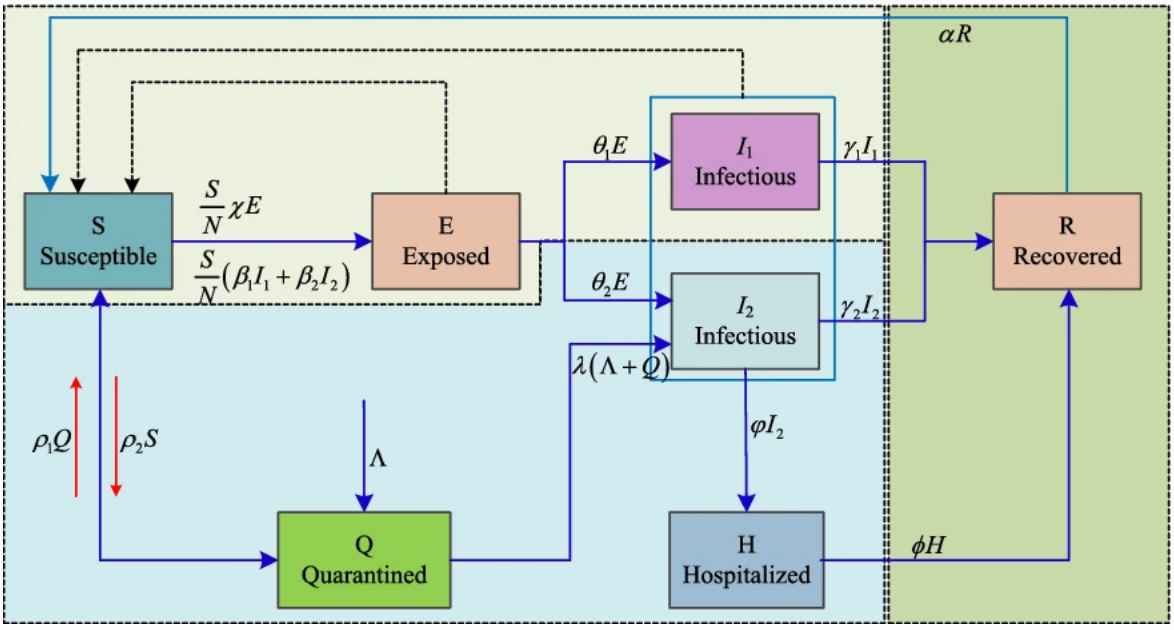
\includegraphics[width=8.5cm]{../Figures/Model_flowchart.png}
    \caption{Diagrama de flujo del modelo}
    \label{block_diagram}
\end{figure}


Como puede verse, el modelo tiene una gran cantidad de parámetros, los cuales deben
ser cuidadosamente seleccionados según las dinámicas de cada región. Por ejemplo, los 
mecanismos de control impuestos por los gobiernos pueden variar en cada país.
\\\\
En el caso del artículo original, se utiliza el algoritmo PSO (\textit{particle swarm optimization})
para estimar los parámetros del modelo de acuerdo a un conjunto de datos de la provincia
de Hubei, en China, de donde también se toman las condiciones iniciales del sistema.
\\\\
La figura \ref{pvi_1} muestra una simulación del problema de valor inicial, utilizando
los mismos parámetros y valores iniciales del artículo.

\begin{figure}[h]
    \centering
    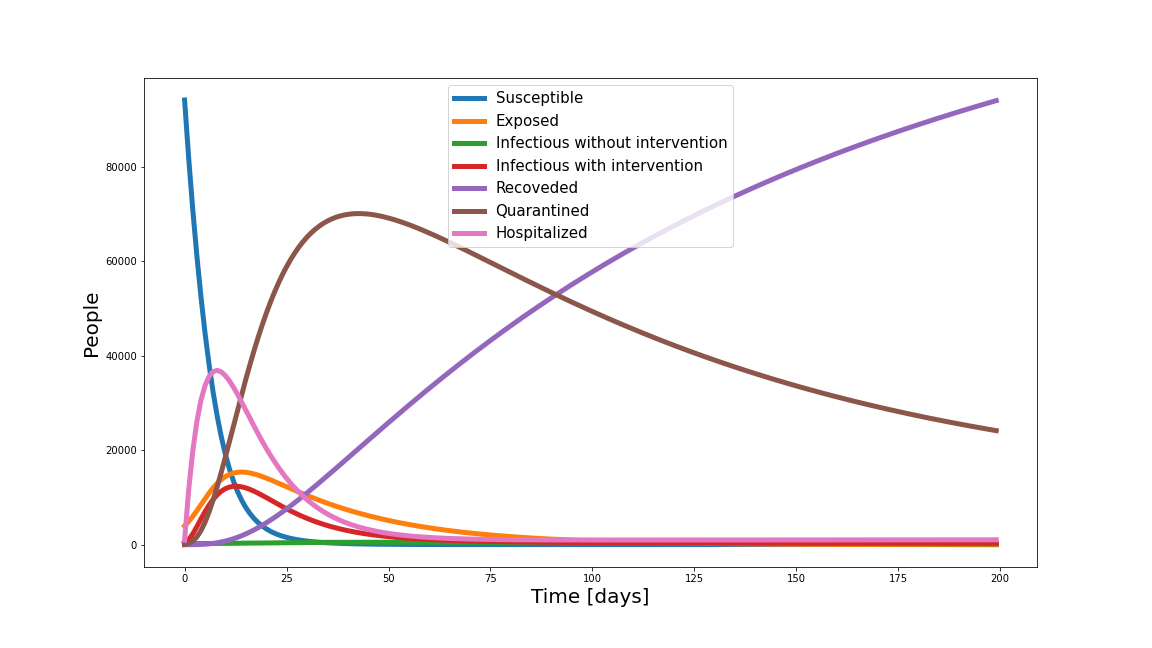
\includegraphics[width=10cm]{../Figures/ivp_1.png}
    \caption{Solución numérica del problema de valores iniciales realizada en Python}
    \label{pvi_1}
\end{figure}

Esta y todas las simulaciones presentadas en este artículo pueden ser consultadas en 
el siguiente enlace: \href{https://github.com/Rmejiaz/ModeladoSimulacion/blob/main/Cuadernos/Proyecto.ipynb}{https://github.com/Rmejiaz/ModeladoSimulacion/blob/main/Cuadernos/Proyecto
.ipynb}

\end{document}
